\documentclass[12pt, a4paper]{article}

\usepackage[utf8]{inputenc}
\usepackage[T2A]{fontenc}
\usepackage[russian]{babel}
\usepackage[dvips]{graphicx}

\usepackage[oglav,spisok,boldsect,eqwhole,figwhole,hyperref,hyperprint,remarks,greekit]{./style/fn2kursstyle}
\graphicspath{{./style/}{./figures/}}
\usepackage{float}
\usepackage{multirow}
\usepackage{supertabular}
\usepackage{multicol}
\usepackage{hhline}
\usepackage{listings}
\usepackage{color}
\usepackage{adjustbox}
\usepackage{amsmath}
\usepackage{verbatim}
\usepackage{amsfonts}
%\usepackage{mathabx}


\definecolor{dkgreen}{rgb}{0,0.6,0}
\definecolor{gray}{rgb}{0.5,0.5,0.5}
\definecolor{mauve}{rgb}{0.58,0,0.82}

\lstset{frame=tb,
	language=C++,
	aboveskip=1mm,
	belowskip=1mm,
	showstringspaces=false,
	columns=flexible,
	basicstyle={\small},
	numbers=left,
	numberstyle=\tiny\color{gray},
	keywordstyle=\color{red},
	commentstyle=\color{dkgreen},
	stringstyle=\color{mauve},
	breaklines=true,
	breakatwhitespace=true,
	tabsize=2
}
\title{Численное решение краевых задач
	для одномерного волнового уравнения \\ Варианты 5, 16}


%\authorfirst{О.\,Д.~Климов}
%\authorsecond{О.\,Д.~Климов} TODO: прописать команды в style.sty

%\supervisor{С.\,А.~Конев}
\supervisor{ }
\group{ФН2-61Б}
\date{2024}

%\renewcommand{\vec}[1]{\text{\mathversion{bold}${#1}$}}%{\bi{#1}}
\newcommand\thh[1]{\text{\mathversion{bold}${#1}$}}
\renewcommand{\labelenumi}{\theenumi)}
\renewcommand{\labelenumi}{\theenumi)}

\newcommand{\opr}{\textbf{\underline{{Опр.}}}\quad}
\newcommand{\theorem}{\textbf{\underline{{Теор.}}}\quad}
\renewcommand{\phi}{\varphi}
\renewcommand{\k}[1]{\textbf{\textit{#1}}}
\newcommand{\widecheck}[1]{\check{#1}}

\newcounter{mycounter}
\newcommand{\quastion}[1]{%
	\stepcounter{mycounter}%
	\textbf{\themycounter}.  %
	\textbf{\textit{#1}}
	
}
\newcommand{\down}[1]{\widecheck{#1}}
\newcommand{\pon}[1]{\mathop {#1}\limits^ \circ}
\newcommand{\rusg}{\text{Г}}

\begin{document}
	\maketitle
	\section{Ответы на контрольные вопросы}
	
	\quastion{Предложите разностные схемы, отличные от схемы "крест" для численного решения задачи (3.1)-(3.4).}
	
	Рассмотрим начально-краевую задачу для волнового уравнения
	
	\begin{equation}
		\begin{cases}
			u_{tt} = a^2 u_{xx}, \quad 0<x<L, \quad 0<t<T, \\
			u(x, 0) = f(x), \\
			u_t(x, 0) = g(x), \\
			u(0,t)=\phi(t), \quad u(L,t) = \psi(t).
		\end{cases}
	\end{equation}
	
	Предложим несколько схем:
	\begin{enumerate}
		\item Трехслойная схема с весами на девятиточечном шаблоне 
		\begin{equation*}
				y_{\bar{t}t} - a^2 (\sigma \hat{y}_{\bar{x}x} + (1 - 2 \sigma) y_{\bar{x}x} + \sigma \widecheck{y}_{\bar{x}x}) = 0
		\end{equation*}
		При выборе постоянного веса схема имеет порядок по крайней мере $O(\tau^2 + h^2)$. А схема с весом $\sigma = \frac{1}{12} - \frac{h^2}{12a^2\tau^2}$ имеет погрешность аппроксимации $O(\tau^4 + h^4)$. Расчет по схеме ведется только при известных значениях $y$ на первых двух временных слоях, где соответственно первое задается начальным условием, а второе рассчитывается по начальному решению и скорости.
		
		\item Двуслойная схема на основе введения скорости. Пусть $v = u_t$. Тогда получаем систему уравнений
		\begin{equation}
			\begin{cases}
				u_t = v,\\
				v_t = a^2 u_{xx}.
			\end{cases}
		\end{equation}
		Тогда можно решить такую задачу с помощью соответствующей двухслойной схемы. Данный подход снимает вопрос о расчете решения на первом временном слое, который не задан начальными данными.
		
		\item Двухслойная схема на основе введения потенциала скорости. Пусть $v = \int_{0}^{x} u_t d\xi$. Тогда исходное уравнение второго порядка сведется к системе уравнений первого порядка
		\begin{equation}
			\begin{cases}
				u_t = v_x,\\
				v_t = a^2 u_x.
			\end{cases}
		\end{equation}
	\end{enumerate}
			
	\quastion{Постройте разностную схему с весами для уравнения колебаний струны. Является ли такая схема устойчивой и монотонной.}
	
	Пусть $u_{tt} \approx y_{\bar{t}t} $ и $u_{xx} \approx y_{\bar{x}x} $. Тогда запишем трехслойную разностную схему
	\begin{equation}
		y_{\bar{t}t} - a^2 (\sigma \hat{y}_{\bar{x}x} + (1 - 2 \sigma) y_{\bar{x}x} + \sigma \widecheck{y}_{\bar{x}x}) = 0
	\end{equation}
	или
	\begin{equation*}
		y_{\bar{t}t} = a^2 (\sigma \hat{y}_{\bar{x}x} + (1 - 2 \sigma) y_{\bar{x}x} + \sigma \widecheck{y}_{\bar{x}x})
	\end{equation*}
	на девятиточечном шаблоне. 
	
	В уравнении схемы входят решения $\widecheck{y}$ и $y$ с известных временных слоев и неизвестное сеточное решение $\hat{y}$.
	
	Очевидно, что при любом постоянном весе $\sigma$ данная схема в силу своей симметричности относительно слоя $t$ имеет порядок аппроксимации по крайней мере $O(\tau^2 + h^2)$. Подбором $\sigma$ можно добиться повышенного порядка аппроксимации. 
	
	Исследуем схему на устойчивость. Обозначим $Ay = a^2 y_{\bar{x}x}$ и воспользуемся равенством
	\begin{equation*}
		\sigma \hat{y} + (1 - 2 \sigma) y + \sigma \widecheck{y} = y + \sigma \tau^2 y_{\bar{t}t}
	\end{equation*}
	Тогда перепишем исходную схему в виде
	\begin{equation*}
		(E - \sigma \tau^2 A)y_{\bar{t}t} = Ay.
	\end{equation*}
	Используем для доказательства энергетический метод. Умножим скалярно уравнение схемы на 
	\begin{equation*}
		y_{\pon{t}} = \frac{y_t + y_{\bar{t}}}{2}. 
	\end{equation*}
	Так как 
	\begin{equation*}
		y_{\bar{t}t} = \frac{y_t - y_{\bar{t}}}{\tau},
	\end{equation*}
	то 
	\begin{equation*}
		(y_{\bar{t}t}, y_{\pon{t}}) = \frac{1}{2} (\parallel y_{\bar{t}} \parallel^2)_t, \quad (A y_{\bar{t}t}, y_{\pon{t}}) = a^2 (y_{\bar{x} \bar{t} t}, y_{\bar{x} \pon{t}}) = - \frac{1}{2} a^2 (\parallel y_{\bar{x} \bar{t}} \parallel^2)_t.
	\end{equation*}
	Последнее равенство следует из формулы интегрирования по частям. Здесь и далее для сокращения записи знак нормы без специального индекса используется для гильбертовой нормы. В частности,
	\begin{equation*}
		\parallel y_{\bar{x} \bar{t}} \parallel = ( y_{\bar{x} \bar{t}},  y_{\bar{x} \bar{t}}).
	\end{equation*}
	 Таким образом, 
	 \begin{equation*}
	 	((R - \sigma \tau^2 A) y_{\bar{t}t}, y_{\pon{t}}) = \frac{1}{2} (\parallel y_{\bar{t}} \parallel^2 + a^2 \sigma \tau^2 \parallel y_{\bar{x}\bar{t}} \parallel^2)_t.
	\end{equation*}
	Преобразуем выражение 
	\begin{equation*}
		(Ay, y_{\pon{t}}) = -a^2 (y_{\bar{x}}, y_{\bar{x} \pon{t}})
	\end{equation*}
	используя формулу Грина, то есть суммирование по частям. Так как для любой сеточной функции справедливы соотношения
	\begin{equation*}
		y = \frac{1}{2} (y^{(0, 5)} +  \down{y}^{(0, 5)} - \frac{1}{2} \tau^2 y_{\bar{t}t}), \quad y_{\pon{t}} = (y^{(0, 5)})_{\bar{t}} = \frac{y_t - y_{\bar{t}}}{2},
	\end{equation*}
	то
	\begin{equation*}
		(Ay, y_{\pon{t}}) = -\frac{1}{2} a^2 (\parallel \down{y}^{(0,5)}_{\bar{x}}\parallel^2)_t + \frac{1}{8} a^2 \tau^2 (\parallel y_{\bar{x}\bar{t}}\parallel^2)_t
	\end{equation*}
	В результате имеем равенство
	\begin{equation*}
		\frac{1}{2}((\parallel y_{\bar{t}} \parallel^2) + \sigma \tau^2 a^2 \parallel y_{\bar{x}\bar{t}} \parallel^2)_t = (-\frac{1}{2} a^2 \parallel y_{\bar{x}} \parallel^2 + \frac{1}{8} a^2 \tau^2 \parallel y_{\bar{x}\bar{t}} \parallel^2)_t 
	\end{equation*}
	то есть
	\begin{equation*}
		\parallel \hat{y} \parallel^2_* = 	\parallel y \parallel^2_*
	\end{equation*}
	где 
	\begin{equation*}
		\parallel y \parallel^2_* = \parallel y_{\bar{t}} \parallel^2 + a^2(\sigma - \frac{1}{4}) \tau^2  \parallel y_{\bar{x}\bar{t}} \parallel^2 + a^2 \parallel \down{y}^{(0,5)}_{\bar{x}}\parallel^2.
	\end{equation*}
	При $\sigma\ge \frac{1}{4}$ величина $\parallel y \parallel_*$ является величиной типа нормы, точнее полунормы --- величины типа нормы, для которой несправедливо первое условие нормы. Рассмотрим другие параметры для чего запишем неравенство типа вложения из метода разделения переменных:
	\begin{equation*}
		\parallel y_{\bar{x}\bar{t}} \parallel^2 \le \frac{4}{h^2} \parallel y_{\bar{t}} \parallel^2.
	\end{equation*}
	Отсюда
	\begin{equation*}
		\parallel y \parallel^2_* \ge (\frac{h^2}{4} + (\sigma - \frac{1}{4}) \tau^2 a^2) \parallel y_{\bar{x}\bar{t}} \parallel^2 + c^2 \parallel \down{y}^{(0,5)}_{\bar{x}}\parallel^2
	\end{equation*}
	Правая часть отрицательна при
	\begin{equation*}
		a^2(\sigma - \frac{1}{4}) \tau^2 + \frac{h^2}{4} \ge 0
	\end{equation*}
	Значит
	\begin{equation*}
		\sigma \ge \frac{1}{4} - \frac{h^2}{4a^2 \tau^2}
	\end{equation*}
	Отсюда видно, что явная схема с $\sigma = 0$ устойчива при $\tau < \frac{h}{a}$, то есть при выполнении критерия Куранта. 
	При выполнении условия устойчивости справедливо неравенство
	\begin{equation*}
		\parallel y \parallel_* \ge a^2 \parallel \down{y}^{(0,5)}_{\bar{x}}\parallel^2
	\end{equation*}
	Из него следует, что с учетом начальных и граничных условий данной задачи величина $\parallel y \parallel_*$ действительно является нормой.  А именно, если $\parallel y \parallel_* = 0$, то $\parallel \down{y}^{(0,5)}_{\bar{x}}\parallel = 0$. Из неравенства вложения $\parallel z \parallel_C \ge \sqrt{l} \parallel z_{\bar{x}} \parallel$ получаем $\down{y}^{(0,5)} = 0$. Это равенство справедливо в силу однородных граничных условий первого рода. Однородные начальные условия дают $y \equiv 0$, следовательно,  $\parallel y \parallel_*$ --- норма.
	
	Из изложенного следует сходимость данной трехслойной разностной схемы со скоростью по крайней мере $O(\tau^2 + h^2)$ при выполнении условия устойчивости
	\begin{equation*}
		\sigma \ge \frac{1}{4} - \frac{h^2}{4a^2 \tau^2}
	\end{equation*}
	
	Исследуем на монотонность. Приведем схему к виду
	\begin{equation*}
		\frac{\hat{y} - 2y + \widecheck{y}}{\tau^2} = a^2 \left( \sigma \frac{\hat{y}_{+1} - 2 \hat{y} + \hat{y}_{-1}}{h^2} + (1 - 2 \sigma) \frac{y_{+1} - 2 y + y_{-1}}{h^2} + \sigma \frac{\widecheck{y}_{+1} - 2 \widecheck{y} + \widecheck{y}_{-1}}{h^2} \right)
	\end{equation*}
	и приведя подобные получим
		\begin{multline*}
			\hat{y}(1 + 2\sigma \frac{a^2 \tau^2}{h^2}) + y (-2 + (1-2\sigma) \frac{a^2 \tau^2}{h^2}) + \down{y}(1 + 2\sigma \frac{a^2 \tau^2}{h^2}) = \\
			=\frac{a^2 \tau^2}{h^2} (\sigma \hat{y}_{+1} + \hat{y}_{-1}) + (1 - 2\sigma)(y_{+1} + y_{-1}) + \sigma( \down{y}_{+1} + \down{y}_{-1}).
		\end{multline*}
	
	Так как коэффициент перед $y$ может быть отрицательным, то не выполняется условие положительности коэффициентов, а значит схема не является чисто монотонной.
	
	\quastion{Предложите способ контроля точности полученного решения.}
	
	Стоит упомянуть, что довольно "робастный" способ --- проводить расчеты на произвольных значениях шагов по сеткам и соответственно изменению вычисленной ошибки уменьшать шаг по определенной сетке. 
	
	Для контроля точности можно использовать аналог правила Рунге. Так как схема имеет порядок $O(\tau^2 + h^2)$, то вычисляя $y^{j+1}$ при шаге $\tau^{j+1}$ и $h^{j+1}$, найдем этот же $y^{j+1}$ при шаге $\frac{\tau^{j+1}}{2}$ и $\frac{h^{j+1}}{2}$. Если норма разности полученных решений меньше заданной нами параметра точности, то решение при шаге $\tau^{j+1}$ и $h^{j+1}$ нас удовлетворяет. В противном случае продолжаем процесс дробления шага до получения необходимой нам точности. Стоит отметить, что данный алгоритм имеет свои недостатки, например при быстрорастущем решении крайне быстро возрастает количество вычислений.
	
	
	
	
	\quastion{Приведите пример трехслойной схемы для уравнения теплопроводности. Как реализовать вычисления по такой разностной схеме? Является ли эта схема устойчивой?}
	
	Рассмотрим задачу вида:
	\[
	\begin{cases}
		u_t = (ku_x)_x, \phantom{xxx} 0<x<l, \phantom{xxx} 0<t<T; \\
		u(x,0) = u_0(x), \\
		u(0,t)=\mu_1(t), \phantom{xxx} u(l,t)=\mu_2(t).
	\end{cases}
	\]
	
	Рассмотрим две схемы.
	\begin{enumerate}
		\item Схема Ричардсона (Крест).
		Выберем шаблон из точек с номерами $(i-1,j)(i, j)(i, j-1)(i, j+1)$ и запишем на нем схему
		\begin{equation*}
			y_{\pon{t}} = k y_{\bar{x}x}
		\end{equation*}
		Схема имеет погрешность аппроксимации $O(\tau^2 + h^2)$, соответствующую наличию центральной разностной производной по времени и второй разностной производной по пространству. Схема является явной. 
		
		Исследуем схему на устойчивость методом гармоник. Подставим в схему решение вида $y_i^j = \rho \exp{(\widetilde{i} i \phi)}$, где $\widetilde{i}$ -- мнимая единица ($\widetilde{i}^2 = -1$). Тогда для определения $\rho$ получим уравнение
		\begin{equation*}
			\frac{\rho-\rho^{-1}}{\tau} = -\frac{8k}{h^2}\sin^2(\frac{\phi}{2}),
		\end{equation*}
		откуда
		\begin{equation*}
		\rho^2 + \frac{8\tau k}{h^2} \sin^2(\frac{\phi}{2}) \rho - 1 = 0.
		\end{equation*}
		Видно, что дискриминант $D = (\frac{4\tau k}{h^2} \sin^2(\frac{\phi}{2}))^2 + 1 gt 0$, следовательно один из корней по модулю заведомо больше единицы. Значит схема является безусловно неустойчивой и непригодной для расчетов.
		\item Cхема Дюфорта-Франкела(Ромб).
		Для построения схемы исключим в предыдущем шаблоне точку $(i, j)$ и заменим в правой части $y$ на $\frac{1}{2}(\hat{y} + \down{y})$. Тогда
		\begin{equation*}
			y_{\pon{t}} = k y_{\bar{x}x} - k \frac{\tau^2}{h^2} y_{\bar{t}t}.
		\end{equation*}
		В таком случае шаблон "Крест" превращается в "Ромб". Нетрудно видеть, что погрешность аппроксимации данной схемы есть величина $O(\tau^2 + h^2 + \frac{tau^2}{h^2})$, то есть является условной. Для обеспечения сходимости параметры $\tau$ и $h$ должны стремится к нулю так, чтобы $\frac{\tau}{h} \to 0$. 
		Исследуем схему на устойчивость методом гармоник. Подставим в схему решение вида $y_i^j = \rho \exp{(\widetilde{i} i \phi)}$, где $\widetilde{i}$ -- мнимая единица ($\widetilde{i}^2 = -1$). Тогда для определения $\rho$ получим уравнение
		\begin{equation*}
			(1 - \frac{4 \tau k}{h^2}) \rho^2 + \frac{4 \tau k} {h^2} \cos(\phi) \rho + (\frac{4 \tau k} {h^2} - 1) = 0.
		\end{equation*}
		Тогда дискриминант $D = 4 - 16 \frac{4 \tau k} {h^2} \sin^2(\phi)$. Выражение для $rho$ имеет вид
		\begin{equation*}
			\rho = \frac{2 \tau k \cos(\phi) \pm \sqrt{h^4 - 4\tau^2 k^2 \sin^2(\phi)}}{h^2 + 4\tau k}.
		\end{equation*}
		По модулю $\rho$ будет заведомо меньше и равен единице, следовательно схема является безусловно устойчивой. 
		
		Стоит отметить, что схема имеет условную аппроксимацию при $\tau < h$.
		
		
		Можно реализовать итерационных процесс по данной схеме таких образом: получить из начальных условий нулевой слой, найти первый временной слой с помощью симметричной схемы и далее использовать трехслойную схему.
	\end{enumerate}
	
	\section{Численные эксперименты}
	
	\subsection{Тест 1}
	\[
	\begin{cases}
		u_{tt} = a^2 u_{xx}, \phantom{xxx} 0<x<L, \phantom{xx} t>0, \\
		u(x,0) = f(x), \phantom{xx} u_t(x,0) = g(x), \phantom{xxx} 0<x<L,\\
		u(0,t) = \varphi(t), \phantom{xx} u(L,t) =\psi(t), \phantom{xxx} t>0.
	\end{cases}
	\]
	
	\textbf{А.} Исходные данные: $f(x)=\sin\pi x$, $g(x)=0$, $\varphi(t)=0$, $\psi(t)=0$, $L=1$, $T= 1$.
	
	Точное решение: $u(x,t) = \sin \pi x \cos \pi t$. Параметры сетки: $h=0.02$, $\tau=0.001$.
	
	\begin{figure}[H]
		\centering
		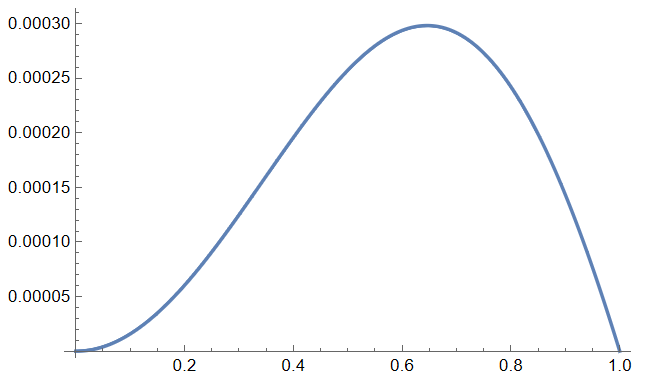
\includegraphics[width=1\textwidth]{errors1}
		\caption{График ошибки численного решения в случае А}
	\end{figure}

	\textbf{Б.} Исходные данные: $f(x)=x(1-x)$, $g(x)=0$, $\varphi(t)=0$, $\psi(t)=0$, $L=1$, $T= 1$.
	
	Точное решение:
	\[
	u(x,t) = \dfrac8\pi \sum_{n=0}^{\infty} \dfrac{1}{(2n+1)^3}\sin(2n+1)\pi x \cos(2n+1)\pi t.
	\]
	 Параметры сетки: $h=0.02$, $\tau=0.001$.
	 
	В качестве точного решения были выбраны слагаемые до номера $k=80$ (требуемая погрешность: $\varepsilon = 10^{-5}$).
	
	\begin{figure}[H]
		\centering
		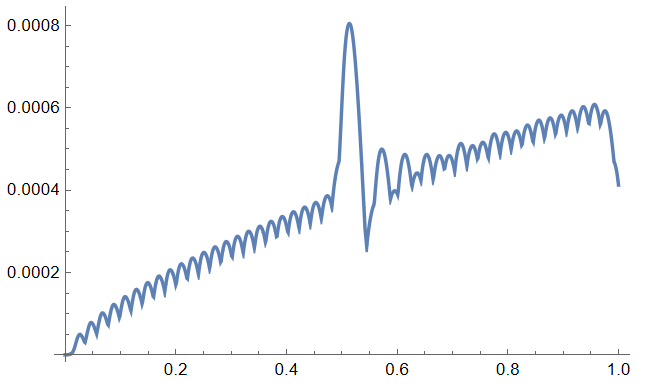
\includegraphics[width=1\textwidth]{errors2}
		\caption{График ошибки численного решения в случае Б}
	\end{figure}

	\clearpage
	\begin{thebibliography}{1}
		\bibitem{1} Галанин М.П., Савенков Е.Б. Методы численного анализа математических моделей. М.: Изд-во МГТУ им. Н.Э. Баумана. 2018. 592 с.
		
	\end{thebibliography}
	
\end{document}